\documentclass[12pt]{article}
\usepackage{amsthm,amssymb,amsmath,amsfonts}
\usepackage[a4paper, top=25mm, bottom=30mm, left=25mm, right=25mm]{geometry}
\usepackage[pagebackref=false,colorlinks,linkcolor=black,citecolor=black]{hyperref}
\usepackage[nameinlink]{cleveref}
 \AtBeginDocument{%
    \crefname{equation}{برابری}{equations}%
    \crefname{chapter}{فصل}{chapters}%
    \crefname{section}{بخش}{sections}%
    \crefname{appendix}{پیوست}{appendices}%
    \crefname{enumi}{مورد}{items}%
    \crefname{footnote}{زیرنویس}{footnotes}%
    \crefname{figure}{شکل}{figures}%
    \crefname{table}{جدول}{tables}%
    \crefname{theorem}{قضیه}{theorems}%
    \crefname{lemma}{لم}{lemmas}%
    \crefname{corollary}{نتیجه}{corollaries}%
    \crefname{proposition}{گزاره}{propositions}%
    \crefname{definition}{تعریف}{definitions}%
    \crefname{result}{نتیجه}{results}%
    \crefname{example}{مثال}{examples}%
    \crefname{remark}{نکته}{remarks}%
    \crefname{note}{یادداشت}{notes}%
    \crefname{observation}{مشاهده}{observations}%
    \crefname{algorithm}{الگوریتم}{algorithms}%
    \crefname{cproof}{برهان}{cproofs}%
}

\usepackage{tikz}
\usepackage{graphicx}
\usepackage{booktabs}
\usepackage{color}
\usepackage{graphicx}
\usepackage{subcaption}

\usepackage{setspace}
\doublespacing

\usepackage{titletoc}
\usepackage{tocloft}
\usepackage{enumitem}
\usepackage{amsmath, amssymb}
\usepackage{algorithm}
\usepackage[noend]{algorithmic}
\renewcommand{\algorithmicrequire}{\textbf{Input:}}
\renewcommand{\algorithmicensure}{\textbf{Output:}}

\usepackage{tabularx}
\makeatletter
\newcommand{\multiline}[1]{%
  \begin{tabularx}{\dimexpr\linewidth-\ALG@thistlm}[t]{@{}X@{}}
    #1
  \end{tabularx}
}
\makeatother

\usepackage{float}
\usepackage{verbatim}
\makeindex
\usepackage{sectsty}
\usepackage{xepersian}
\SepMark{-}
\settextfont[Scale=1.2,Path=fonts/,BoldFont=B Nazanin Bold.ttf]{B Nazanin.ttf}
\setlatintextfont{Times New Roman}
\renewcommand{\labelitemi}{$\bullet$}

\theoremstyle{definition}
\newtheorem{definition}{تعریف}[section]
\newtheorem{remark}[definition]{نکته}
\newtheorem{note}[definition]{یادداشت}
\newtheorem{example}[definition]{نمونه}
\newtheorem{question}[definition]{سوال}
\newtheorem{remember}[definition]{یاداوری}
\newtheorem{observation}[definition]{مشاهده}
\theoremstyle{theorem}
\newtheorem{theorem}[definition]{قضیه}
\newtheorem{lemma}[definition]{لم}
\newtheorem{proposition}[definition]{گزاره}
\newtheorem{corollary}[definition]{نتیجه}
\newtheorem*{cproof}{برهان}




\begin{document}
\fontsize{12pt}{14pt}\selectfont

\begin{minipage}{0.1\textwidth}

\includegraphics[width=3cm]{etc/IUST}
\end{minipage}%
\hfill%
\begin{minipage}{0.6\textwidth}\centering
\fontsize{13pt}{13pt}\selectfont
به‌ نام خدا \\
\textbf{درس یادگیری عمیق} \\
\textbf{تمرین سری ششم}\\
استاد درس : دکتر محمدرضا محمدی \\
دستیاران :  مهدی خورشا، سید محمد موسوی،\\ امیرحسین نمازی
\\
\vspace{0.25cm}
\begingroup
\fontsize{11pt}{11pt}\selectfont
دانشگاه علم و صنعت ایران، دانشکده مهندسی کامپیوتر \\
نیمسال دوم تحصیلی 1403 - 1404 \\
\endgroup
\end{minipage}%
\hfill%
\begin{minipage}{0.1\textwidth}

\end{minipage}

\vspace{0.5cm}

\noindent\rule{\textwidth}{1pt}

\centering {\fontsize{18}{22}\selectfont \textbf{مهلت تحویل : 1404/01/15 }}\\
{\fontsize{14}{22}\selectfont \textbf{لطفا به نکات موجود در سند قوانین انجام و تحویل تمرین ها دقت فرمایید. }}

\begin{enumerate}

    \section*{سوالات تئوری}
    \item 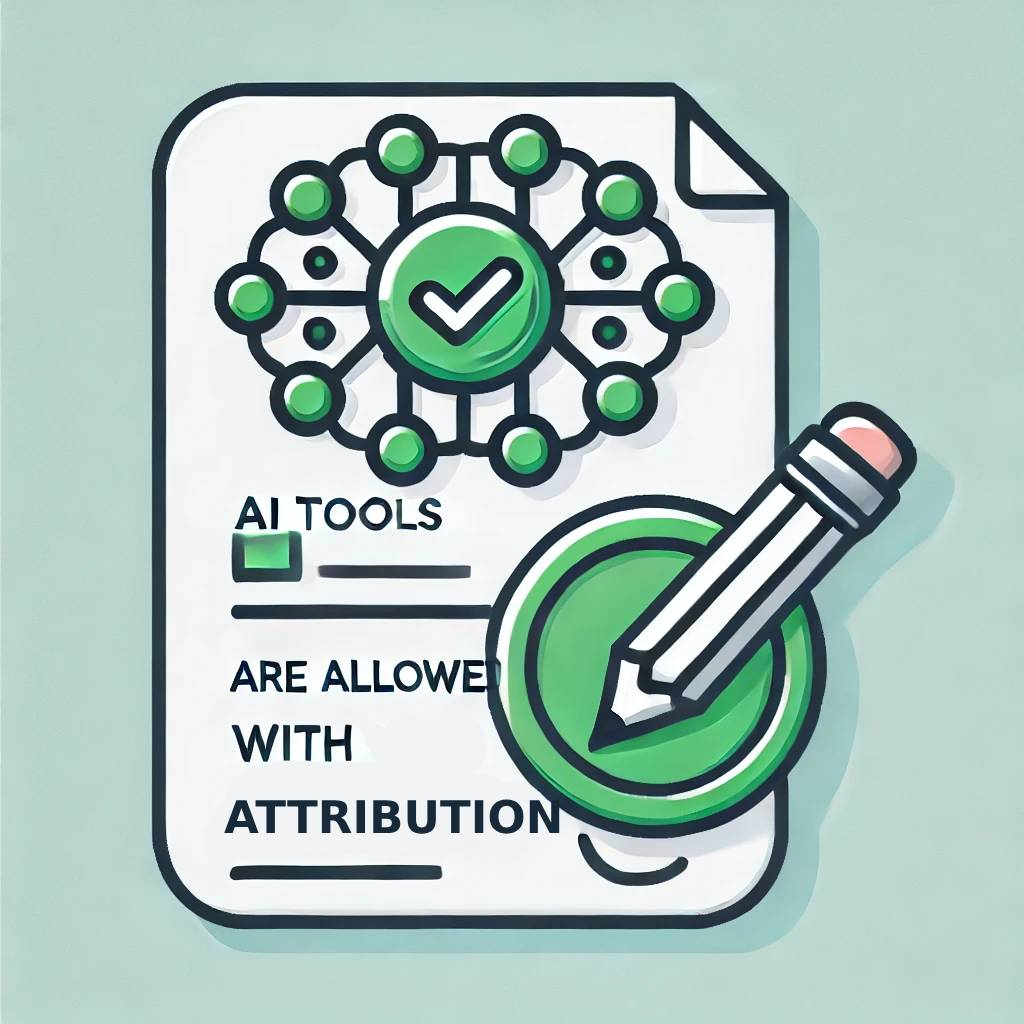
\includegraphics[width=1cm]{figs/Allowed_with_contributino.jpg}
     ابتدا مقاله \href{https://arxiv.org/pdf/2208.03608}{\lr{\textbf{Shap-CAM}}} را مطالعه کنید و سپس به سوالات زیر پاسخ دهید(10نمره).\\
     \begin{enumerate}
         \item روش‌های \lr{\textbf{Grad-CAM}} و \lr{\textbf{Shap-CAM}} را از نظر ویژگی‌های زیر مقایسه کنید:
         \begin{itemize}
             \item نحوه محاسبه اهمیت ویژگی‌ها (ویژگی‌های محلی یا جهانی)\\
             \textcolor{blue}{
             \lr{\textbf{Shap-CAM}}: این روش اهمیت هر پیکسل را با تخمین سهم حاشیه‌ای آن در خروجی مدل (اطمینان\LTRfootnote{Confidence} از کلاس) تعیین می‌کند. برای این کار، مفهوم مقدار شاپلی\LTRfootnote{Shapley} از نظریه بازی‌های مشارکتی\LTRfootnote{Cooperative} معرفی شده است. مقدار شاپلی برای یک پیکسل با در نظر گرفتن سهم آن در تمام زیرمجموعه‌های ممکن محاسبه می‌شود. این فرآیند به طور ذاتی روابط و تعاملات بین پیکسل‌های مختلف را لحاظ می‌کند. این روش یک نسبت‌دهی در سطح ویژگی ارائه می‌دهد که سهم کلی ویژگی‌های ورودی را مشخص می‌کند.}\\
             \textcolor{blue}{
            \lr{\textbf{Grad-CAM}}: این یک روش مبتنی بر گرادیان است که اهمیت هر کانال از نقشه‌های فعال‌سازی لایه نهایی کانولوشن را با استفاده از گرادیان اطمینان کلاس نسبت به این نقشه‌ها محاسبه می‌کند. این گرادیان‌ها نشان می‌دهند که هر مکانی چقدر به پیش‌بینی کلاس کمک می‌کند. نقشه نهایی برجستگی، یک جمع وزنی از نقشه‌های فعال‌سازی است. \lr{\textbf{Grad-CAM}} توضیحات مکانی ارائه می‌دهد و مناطقی از فعال‌سازی بالا را که به نواحی مهم در ورودی مربوط هستند، برجسته می‌کند. این روش سهم را براساس فعال‌سازی می‌سنجد، اما مانند مقدار شاپلی به طور صریح تعامل بین ویژگی‌ها یا پیکسل‌ها را در نظر نمی‌گیرد. \lr{\textbf{Grad-CAM}} فاقد دقت و جزئیات اهمیت فردی ویژگی‌هاست که روش‌های مبتنی بر شاپلی فراهم می‌کنند.}
            
             \item وابستگی به ساختار مدل و نیاز به گرادیان:\\
             \textcolor{blue}{
             \lr{\textbf{Shap-CAM}}: یک روش توضیح بصری پساحسابی\LTRfootnote{post-hoc} است. ویژگی کلیدی این روش این است که وابستگی به گرادیان‌ها را حذف می‌کند. این روش یک رویکرد بدون گرادیان است که اهمیت پیکسل را از طریق مقدار شاپلی به‌دست می‌آورد، نه از طریق گرادیان‌ها. این به این معناست که عملکرد آن به پایداری یا قابلیت اعتماد گرادیان‌ها وابسته نیست.}\\
             \textcolor{blue}{
            \lr{\textbf{Grad-CAM}}: نیز یک روش پساحسابی است. این روش اساساً یک رویکرد مبتنی بر گرادیان است. این روش به گرادیان‌هایی که از طریق پس‌انتشار محاسبه می‌شوند، برای ترکیب نقشه‌های ویژگی کانولوشنی تصحیح‌شده\LTRfootnote{Rectified}، متکی است. \lr{\textbf{Grad-CAM}} گرادیان‌ها را به‌عنوان میزان اهمیت هر کانال نسبت به احتمال کلاس در نظر می‌گیرد. این به این معناست که برای دسترسی به گرادیان‌های خروجی مدل نسبت به نقشه‌های ویژگی لایه کانولوشنی نیاز دارد و به آن‌ها وابسته است.}
            
             \item دقت در شناسایی نواحی مهم تصویر:\\
             \textcolor{blue}{
             \lr{\textbf{Shap-CAM}}: عملکرد بصری بهتر و عدالت بیشتری در تفسیر فرآیند تصمیم‌گیری نسبت به روش‌های موجود نشان می‌دهد. به دلیل برتری مقدار شاپلی و توجه آن به روابط بین پیکسل‌ها، \lr{\textbf{Shap-CAM}} توضیحات منطقی‌تر و دقیق‌تری از سهم هر پیکسل ارائه می‌دهد. از نظر کیفی، \lr{\textbf{Shap-CAM}} نقشه‌های برجستگی هموارتر و با نویز تصادفی کمتری نسبت به روش‌های مبتنی بر گرادیان تولید می‌کند. از نظر کمی نیز در وظایف شناسایی (کاهش بیشتر \lr{Average Drop} و افزایش بیشتر \lr{Average Increase}) و وظایف مکان‌یابی (نسبت بالاتر) عملکرد بهتری نسبت به روش‌های قبلی مانند \lr{\textbf{Grad-CAM}} و \lr{Grad-CAM++} دارد. این نتایج نشان می‌دهد که \lr{\textbf{Shap-CAM}} می‌تواند فرآیند تصمیم‌گیری مدل را با دقت بیشتری آشکار کند و نقشه‌های برجستگی تولیدشده نویز کمتری دارند.}\\
             \textcolor{blue}{
            \lr{\textbf{Grad-CAM}}: شفافیت مدل‌های \lr{CNN} را با نمایش نواحی ورودی مهم برای پیش‌بینی بهبود بخشید. با این حال، روش‌های مبتنی بر گرادیان مانند \lr{\textbf{Grad-CAM}} به دلیل فرضیه‌های اثبات‌نشده در مورد وزن‌های نقشه‌های فعال‌سازی، نمی‌توانند اطلاعات اصیل\LTRfootnote{Authentic} را به درستی نمایش دهند. این روش‌ها فاقد پایه نظری مستحکم بوده و به عنوان روش‌هایی توصیف شده‌اند که به اندازه کافی مقاوم\LTRfootnote{Robust} و قابل اعتماد نیستند.
             }
             \item حساسیت به تغییرات کوچک در ورودی:\\
             \textcolor{blue}{
             \lr{\textbf{Shap-CAM}}: مقالات اشاره می‌کنند که روش‌های مبتنی بر گرادیان مانند \lr{\textbf{Grad-CAM}} می‌توانند به راحتی توسط دستکاری‌های مخرب مدل که گرادیان‌ها را بدون ایجاد تغییرات محسوس در تصویر تغییر می‌دهند، فریب داده شوند. در مقابل، \lr{\textbf{Shap-CAM}} می‌تواند اثر این مشکل را کاهش دهد، زیرا اهمیت پیکسل‌ها را با دقت بیشتری تخمین می‌زند؛ بخشی از این دقت به دلیل پایداری مفهوم مقدار شاپلی و توجه آن به روابط بین پیکسل‌هاست.}\\
             \textcolor{blue}{
             \lr{\textbf{Grad-CAM}}: روش‌های مبتنی بر گرادیان برای تولید نقشه‌های کلاس-فعال‌سازی به عنوان روش‌هایی توصیف شده‌اند که به اندازه کافی مقاوم و قابل اعتماد نیستند. این روش‌ها می‌توانند به راحتی با تغییر گرادیان‌ها بدون تغییرات محسوس در تصاویر اصلی فریب داده شوند. این موضوع نشان‌دهنده حساسیت این روش‌ها به تغییرات کوچک ورودی است که می‌تواند گرادیان‌ها را به طور قابل توجهی تحت تأثیر قرار دهد.
             }
         \end{itemize}
         \textbf{برای پاسخ به این بخش میتوانید از این \href{https://arxiv.org/pdf/2412.16003}{مقاله} استفاده کنید.}
         \vspace{1cm}
         \item فرض کنید مدلی که برای طبقه‌بندی تصاویر استفاده می‌کنید، نسبت به تغییرات ناچیز در ورودی حساس است.
         \begin{itemize}
             \item آیا انتظار دارید \lr{\textbf{Grad-CAM}} و \lr{\textbf{Shap-CAM}} رفتار مشابهی داشته باشند؟ چرا؟\\
             \textcolor{blue}{
             ما لزوماً انتظار نداریم که \lr{\textbf{Shap-CAM}} و \lr{\textbf{Grad-CAM}} رفتار مشابهی داشته باشند، به‌ویژه زمانی که حساسیت مدل ناشی از تغییرات کوچک ورودی و تأثیر آن‌ها بر گرادیان‌ها باشد.
            \lr{\textbf{Grad-CAM}} یک روش مبتنی بر گرادیان است که اهمیت ویژگی‌ها را با استفاده از گرادیان‌های اعتماد به کلاس نسبت به نقشه‌های فعال‌سازی تعیین می‌کند. مقالات اشاره می‌کنند که روش‌های مبتنی بر گرادیان مقاومت کافی ندارند و می‌توانند با دستکاری گرادیان‌ها بدون تغییر محسوس تصویر فریب داده شوند. بنابراین، اگر تغییرات کوچک ورودی گرادیان‌ها را به‌شدت تحت تأثیر قرار دهد، توضیحات \lr{\textbf{Grad-CAM}} نیز ناپایدار خواهند بود.
            \lr{\textbf{Shap-CAM}}، در مقابل، روشی بدون استفاده از گرادیان است که اهمیت پیکسل‌ها را بر اساس مقدار شاپلی تخمین می‌زند و تعاملات بین پیکسل‌ها را در نظر می‌گیرد. چون به گرادیان‌ها وابسته نیست، حساسیت آن به پایداری گرادیان‌های مدل مرتبط نیست و توضیحات پایدارتر و دقیق‌تری ارائه می‌دهد.
            در نتیجه، در شرایطی که حساسیت مدل به رفتار گرادیان‌ها مربوط باشد، \lr{\textbf{Shap-CAM}} می‌تواند نسبت به \lr{\textbf{Grad-CAM}} توضیحاتی پایدارتر و قابل اعتمادتر ارائه کند.
             }
             \item کدام روش می‌تواند پایداری بیشتری داشته باشد؟ توضیح دهید.\\
             \textcolor{blue}{
             بر اساس مقالات، انتظار می‌رود که \lr{\textbf{Shap-CAM}} در مواجهه با حساسیت مدل نسبت به تغییرات کوچک ورودی، پایدارتـر عمل کند.
            شواهدی که مقالات برای پایداری بیشتر \lr{\textbf{Shap-CAM}} ارائه داده‌اند شامل موارد زیر است:
            روش‌های مبتنی بر گرادیان، از جمله \lr{\textbf{Grad-CAM}}، به عنوان «غیرمقاوم و غیرقابل اعتماد» توصیف شده‌اند.
            این روش‌ها «به راحتی می‌توانند با دستکاری گرادیان‌ها بدون تغییر محسوس تصویر فریب داده شوند»، که نشان‌دهنده ناپایداری در برابر تغییرات ورودی است که بر گرادیان‌ها اثر می‌گذارند.
            در مقابل، \lr{\textbf{Shap-CAM}} با استفاده از مقدار شاپلی، وابستگی به گرادیان‌ها را حذف می‌کند.
            مقدار شاپلی، مفهومی از نظریه بازی‌های مشارکتی با پایه نظری قوی و ویژگی‌هایی چون کارایی \LTRfootnote{Efficiency} است که تعامل بین ویژگی‌ها را نیز در نظر می‌گیرد و می‌تواند توضیحات منطقی‌تر و دقیق‌تری ارائه کند.
            مقالات بیان می‌کنند که \lr{\textbf{Shap-CAM}} می‌تواند «اثر این مشکل» (دستکاری گرادیان‌ها) را کاهش دهد و اهمیت پیکسل‌ها را دقیق‌تر تخمین بزند.
            به صورت کیفی، \lr{\textbf{Shap-CAM}} نقشه‌های برجستگی \LTRfootnote{saliency maps} صاف‌تر و با نویز کمتری نسبت به روش‌های مبتنی بر گرادیان تولید می‌کند که می‌تواند نشانه‌ای از پایداری بیشتر باشد.
             }
         \end{itemize}
     \end{enumerate}
     \vspace{1cm}

    \item 
\includegraphics[width=1cm]{figs/Forbidden_AI.jpg}
    به سوالات زیر در مورد شبکه های عصبی پیچشی\LTRfootnote{Convolutional} پاسخ دهید(10 نمره)\\
    \begin{enumerate}
        \item مفهوم به اشتراک‌گذاری پارامترها در شبکه‌های عصبی پیچشی چیست و چه تاثیری در روند آموزش مدل دارد؟\\
        \textbf{در پاسخ این قسمت از فایل آقای حسین‌زاده استفاده شده است}\\
        \textcolor{blue}{
        در شبکه‌های عصبی پیچشی، از فیلترهایی استفاده می‌شود که در سراسر تصویر حرکت می‌کنند (عملیات کانولوشن). این فیلترها دارای مجموعه ای از وزن ها (پارامترها) هستند که در کل تصویر یکسان باقی می‌مانند. اگر می‌خواهیم یک ویژگی را تشخیص بدهیم، می‌توانیم از همان آشکارساز در گوشه پایین سمت چپ تصویر و در سمت راست بالای تصویر استفاده کنیم. در شبکه‌های \lr{Fully Connected}، هر نورون به همه‌ی ورودی‌ها وصل است و وزن مخصوص به خودش را دارد. ولی در \lr{CNN}  به خاطر به اشتراک‌گذاری، تعداد وزن‌ها خیلی کمتر می‌شود. در واقع این ویژگی باعث می‌شود سرعت یادگیری بیشتر شود چون تعداد وزن‌هایی که باید به روزرسانی شوند کمتر است. هم‌چنین مدل سبک‌تر شده و حافظه کمتری مصرف می‌شود. به‌علاوه مدل باید سعی کند ویژگی‌هایی را یاد بگیرد که در کل تصویر کاربرد دارد بنابراین پایداری و\lr{generalization}  هم افزایش میابد.
        }
        \item توضیح دهید برای هریک از سناریوهای زیر شبکه‌های عصبی پیچشی مناسب هستند یا خیر:
        \begin{itemize}
            \item نظارت بر یک گونه‌ی خاص از گرگ در حیات وحش با پهپاد:\\
            \textbf{در پاسخ این قسمت از فایل آقای مرادی استفاده شده است}\\
            \textcolor{blue}{
            بله، زیرا \lr{CNN}ها در تشخیص اشیا و دسته بندی تصاویر، به دلیل داشتن فیلترهای متفاوت برای یافتن الگوهایی ویژه (مانند رنگ بدن، شکل گوش و ...)، توانایی بالایی دارند و برای شناسایی حیوانات در تصاویر طبیعی بسیار مناسب‌اند.
            }
            \item استخراج متن از درون صوت:\\
            \textbf{در پاسخ این قسمت از فایل آقای مرادی استفاده شده است}\\
            \textcolor{blue}{
            بله، زیرا شبکه‌های عصبی کانولوشنی این قابلیت را دارند که با استفاده از فیلترها و عملیات ریاضی کانولوشن، الگوهای محلی موجود در سیگنال صوتی را که مربوط به کلمات خاصی هستند، شناسایی کنند. به این ترتیب، می‌توانند کلمه به کلمه اطلاعات را استخراج کرده و در نهایت جمله‌ی کامل را بسازند. اما نکته‌ی منفی این روش این است که برای پوشش طیف وسیعی از کلمات و تلفظ‌ها، باید تعداد زیادی فیلتر آموزش ببینند تا مدل بتواند تفاوت‌های ظریف بین کلمات را تشخیص دهد.}
            \item شناسایی عمل انجام شده درون ویدیو:\\
            \textcolor{blue}{
            شبکه‌های \lr{CNN} برای انجام این وظیفه مناسب نیستند. زیرا تشخیص نوع حرکت در طول چندین فریم، یک مسئله‌ی نیازمند حافظه است که با روش‌هایی مانند \lr{RNN} یا \lr{Transformer} که دارای قابلیت به یاد سپاری در طول یک دنباله هستند قابلیت حل دارد. شبکه‌های \lr{CNN} تنها می‌توانند نقش استخراج ویژگی از روی فریم‌های یک ویدیو برای پردازش در مراحل بعد را بازی کنند. (شبکه‌های \lr{CNN} سه‌بعدی در تئوری برای این وظیفه مناسب هستند و می‌توانند آن را حل کنند اما به دلیل سنگین بودن این نوع مدل‌ها، نیاز شدید به دیتای زیادی که خاص منظوره برچسب خورده‌اند و نیز هزینه‌ی زیاد در هنگام استنتاج به دلیل پردازش پنجره‌ی ثابتی از فریم‌های متوالی از منظر عملی مناسب و بهینه نبوده و نیز دارای دقت پایینی هستند)
            }
            \item داوری انجام حرکت میل‌زنی در مسابقات زورخانه‌ای:\\
            \textcolor{blue}{
            برای این وظیفه مناسب هستند. باتوجه به نوع داوری مسابقات میل‌زنی که براساس زاویه‌ی دست، بدن، میل و هم‌چنین برخورد میل با سر و ... انجام می‌شود شبکه‌های عصبی \lr{CNN} می‌توانند مناسب باشند. برای انجام آن کافی است با روش‌های \lr{pose estimation} نقاط مشخصه بدن (\lr{landmark}) در لحظه‌ای خاص را استخراج کنیم و سپس از روی این نقاط یافتن زاوایای دست، آرنج، بازو و ... به‌راحتی قابل استخراج است.
            }
        \end{itemize}
        \item معادله‌ی تلفیق (\lr{fusion}) لایه‌ی \lr{batchNorm2D} درون یک لایه‌ی \lr{Conv2D} را بنویسید و توضیح دهید این عمل چه تاثیری در عملکرد مدل دارد.\\
        \textbf{در پاسخ این قسمت از فایل خانم میاهی‌نیا استفاده شده است}\\
        \textcolor{blue}{
        در واقع، لایه‌ی کانولوشن دو بعدي هم يک عمليات خطي هست، خيلي شبيه به لایه‌ي \lr{FC}، ولي با اشتراک‌گذاري وزن‌ها و ساختار مکاني. ما مي‌توانیم کانولوشن رو به شکل زير بازنويسي کنيم:
           $$Z = W * X + b$$
        درحالی که \lr{W} يک کرنل کانولوشني، \lr{b}  باياس و \lr{X}  ورودي مي‌باشد.
        از طرفي فرمول \lr{batch normalization}:
        $$y = \gamma \times \frac{Z - \mu}{\sqrt{\sigma^2 + \epsilon}} + \beta$$
        معادله تلفيق آن را مي‌توان به صورت زير نوشت:
        $$W_{\text{\lr{fused}}} = \gamma \times \frac{W}{\sqrt{\sigma^2 + \epsilon}}$$
        $$b_{\text{\lr{fused}}} = \gamma \times \frac{b - \mu}{\sqrt{\sigma^2 + \epsilon}} + \beta$$
        $$Y = W_{\text{\lr{fused}}} \times X + b_{\text{\lr{fused}}}$$
        ترکيب کردن لایه‌ها مثل \lr{Conv2D + BatchNorm}  باعث مي‌شود اين عمليات‌ها به جاي اجرا به‌صورت جداگانه، به‌صورت يک عمليات واحد روي سخت افزار اجرا بشوند. يعني، کاهش تعداد دفعات دسترسي به حافظه، کاهش زمان اجراي کل شبکه و مناسب براي اجرا روي \lr{GPU} هاي محدود.
        اين عمليات‌هاي ترکيب‌شده هيچ اثري روي دقت مدل ندارند زيرا عمليات‌هاي \lr{Conv}  و \lr{BatchNorm}  خطي 
        هستند و مي‌توانند به صورت رياضياتي ترکيب بشوند و فقط ساختار گراف تغيير مي‌کند، نه منطق مدل يا وزن‌هاي آموزش ديده.
        }
        \item یکی از کاربردهای مدل‌های چندوجهی\LTRfootnote{Multi-Modal}  مانند \lr{ChatGPT} وظیفه‌ی \lr{VQA}\LTRfootnote{Visual question answering}  (پرسش و پاسخ تصویر) است. در این وظیفه مدل تصویر و سوالی درباره‌ی تصویر از کاربر می‌گیرد و باید جواب متناسبی برای آن تولید کند. یکی از نقاط ضعف این مدل‌ها، پاسخ دادن به سوالاتی است که از جزئیات ریز و درحاشیه‌ی تصویر پرسیده می‌شوند. این نوع مدل‌ها در پاسخ به سوالات مربوط به تصویر حاوی یک شی برجسته در وسط توانایی خوبی دارند. برای پوشش دادن این ضعف یکی از کارهایی که می‌توان کرد، تشخیص درست ناحیه‌ی مورد پرسش و برش آن برای ورود به مدل است. فرض کنید ما یک مدل \lr{Question-image matching} توسعه داده‌ایم. اما این مدل تنها میان مفهوم کلی سوالات ورودی و تصویر انطباق انجام می‌دهد و درباره‌ی ناحیه‌ی آن اشاره‌ای نمی‌کند. با استفاده از مفاهیمی که تاکنون خوانده‌اید راه‌حلی برای این مسئله پیشنهاد دهید.\\
        \textcolor{blue}{
        این سوال از روی ایده‌ی مقاله‌ی \href{https://arxiv.org/abs/2212.10846}{\lr{Img2LLM}} طرح شده است.
        همانطور که در شکل زیر که نمایی کلی از متد پیشنهادی مدل مقاله‌ی ذکر شده است، با استفاده از \lr{GradCAM} بر روی \lr{attention map} های مدل \lr{question-image matching} می‌توانند به ناحیه‌ی حدودی از تصویر که سوال ورودی به آن مربوط است برسند. البته لازم به ذکر است که این مقاله برای بهبود عملکرد مدل نهایی ایده‌ی خوب دیگری داشته است که در اسکوپ این تمرین نیست و خواننده‌های علاقه‌مند را به مطالعه‌ی مقاله‌ی سایت شده ارجاع می‌دهیم.}\\
        \begin{figure}[h]  
            \centering
            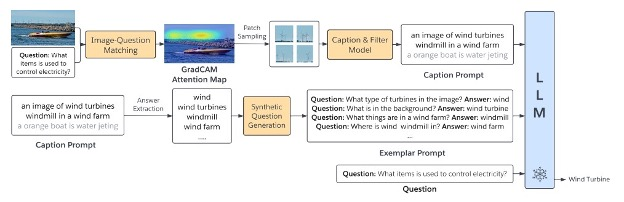
\includegraphics[width=\textwidth]{figs/Q2_d.jpg}
        \end{figure}
        \textcolor{blue}{
        دلیل اینکه \lr{Attention map} های مدل \lr{QIM} می‌توانند به ناحیه‌ای از تصویر توجه کنند که سوال بیشتر مربوط به آن ناحیه است، یادگیری فضای بازنمایی مشترک میان متن و تصویر از نوع آموزش چندوجهی آن است. 
        توجه:
        پاسخ این سوال یکتا نیست و پاسخ فوق تنها نمونه‌ای از آن‌ها و پیشنهاد ما می‌باشد. برای نمره‌دهی این سوال حتما به میزان منطقی و عملیاتی بودن پاسخ‌های دانشجویان اهمیت داده خواهد شد.}
    \end{enumerate}
    \newpage
    \item 
\includegraphics[width=1cm]{figs/Forbidden_AI.jpg}
    تعداد پارامتر، ضرب و جمع و هم‌چنین میدان دید موثر لایه‌های شبکه‌ی عصبی با ورودی تصاویر رنگی از ابعاد 256 در 256 زیر را به تفصیل محاسبه کنید (لطفا اعداد اعشاری را به پایین گرد کنید)(15 نمره)\\
    
        \lr{
        {\ttfamily  
            \begin{itemize}
                \item \textbf{Layer1 : nn.Conv2d(in\_channels=3, out\_channels=32, kernel\_size=(7,7), stride=1, padding='same')}
                \item \textbf{bn1 : nn.BatchNorm2d(32)}
                \item \textbf{Layer2 : nn.Conv2d(in\_channels=32, out\_channels=64, kernel\_size=(5,5), stride=2, padding='valid')}
                \item \textbf{bn2 : nn.BatchNorm2d(64)}
                \item \textbf{Layer3 : nn.AvgPool2d(kernel\_size=(2,2), stride=2)}
                \item \textbf{Layer4 : nn.Conv2d(in\_channels=64, out\_channels=128, kernel\_size=(3,3), stride=1, dilation=2, padding='valid')}
                \item \textbf{bn3 : nn.BatchNorm2d(128)}
                \item \textbf{Layer5 : nn.Conv2d(in\_channels=128, out\_channels=128, kernel\_size=(3,3), stride=1, dilation=1, padding='valid')}
                \item \textbf{bn4 : nn.BatchNorm2d(128)}
                \item \textbf{Layer6 : nn.AvgPool2d(kernel\_size=(2,2), stride=2)}
                \item \textbf{Layer7 : nn.Conv2d(in\_channels=128, out\_channels=256, kernel\_size=(3,3), stride=1, padding='valid')}
                \item \textbf{bn5 : nn.BatchNorm2d(256)}
                \item \textbf{Layer8 : nn.AvgPool2d(kernel\_size=(2,2), stride=2)}
                \item \textbf{fc1 : nn.Linear(in\_features=43264, out\_features=1024)}
                \item \textbf{fc2 : nn.Linear(in\_features=1024, out\_features=1024)}
                \item \textbf{dropout : nn.Dropout(p=0.5)}
                \item \textbf{fc3 : nn.Linear(in\_features=1024, out\_features=10)}
            \end{itemize}
            } }
            
    \textcolor{blue}{
    ابتدا تعداد پارامترهای هر لایه را محاسبه می‌کنیم. سپس به سراغ \lr{receptive field}  لایه‌ها می‌رویم. فرمول محاسبه پارامترها:\\\\
    لایه‌ی کانولوشن:
    $$\text{\lr{num\_filters}} \times (\text{\lr{kernel\_size}} \times \text{\lr{kernel\_size}} \times \text{\lr{num\_in\_channels}} + 1)$$
    لایه \lr{batch norm}:\\\\
     برای هر چنل، 2 پارامتر یادگیری دارد پس\\\\ 
    $$\text{\lr{num\_channel}} \times 2$$
    لایه‌ی \lr{FC}:\\
    $$\text{\lr{output\_size}} \times (\text{\lr{input\_size}} + 1)$$
    \textbf{تعداد پارامترها:}\\
    \lr{
        \begin{enumerate}
            \item Conv1: \( 32 \times (1 + 3 \times 7 \times 7) = 4736 \)
            \item bn1: \( 32 \times 2 = 64 \)
            \item Conv2: \( 64 \times (1 + 32 \times 5 \times 5) = 51264 \)
            \item bn2: \( 64 \times 2 = 128 \)
            \item Conv3: \( 128 \times (1 + 64 \times 3 \times 3) = 73856 \)
            \item bn3: \( 128 \times 2 = 256 \)
            \item Conv4: \( 128 \times (1 + 128 \times 3 \times 3) = 147584 \)
            \item bn4: \( 128 \times 2 = 256 \)
            \item Conv5: \( 256 \times (1 + 128 \times 3 \times 3) = 295168 \)
            \item bn5: \( 256 \times 2 = 512 \)
            \item fc1: \( 1024 \times (43264 + 1) = 44303360 \)
            \item fc2: \( 1024 \times (1024 + 1) = 1049600 \)
            \item fc3: \( 10 \times (1024 + 1) = 10250 \)
        \end{enumerate}
    }
    مجموعا حدودا 45.9 میلیون پارامتر \\
    \textbf{میدان‌دید لایه‌ها (منبع:  \lr{Stanford CS231n}):}\\
    میدان‌دید هر لایه از طریق فرمول زیر محسابه می‌شود:
    $$
    R_i = R_{i-1} + (k_i - 1) \cdot d_{i} \cdot j_{i-1}
    $$
    $$
    j_{i} = j_{i-1} \cdot s_{i}
    $$\\
    که \( R_{i-1} \) میدان‌دید لایه قبلی، \( j_{i-1} \) به‌عنوان پرش از لایه قبلی به لایه فعلی، \( k_i \) اندازه کرنل و \( d_i \) نیز \lr{stride} همان لایه است.\\
    $$
    d_{i} = \text{\lr{dilataion}}, R_{0}=j_{0}=1
    $$
    \lr{
    \begin{enumerate}
        \item Conv1: \( 7 \times 7 \), \( k_1 = 7 \), \( d_1 = 1 \), \( j_1 = 1 \)
        \item Conv2: \( 11 \times 11 \), \( k_2 = 5 \), \( d_2 = 1 \), \( j_2 = 2 \)
        \item AvgPool1: \( 13 \times 13 \), \( k_3 = 2 \), \( d_3 = 1 \), \( j_3 = 4 \)
        \item Conv3: \( 29 \times 29 \), \( k_4 = 3 \), \( d_4 = 2 \), \( j_4 = 4 \)
        \item Conv4: \( 37 \times 37 \), \( k_5 = 3 \), \( d_5 = 1 \), \( j_5 = 4 \)
        \item AvgPool2: \( 41 \times 41 \), \( k_6 = 2 \), \( d_6 = 1 \), \( j_6 = 8 \)
        \item Conv5: \( 57 \times 57 \), \( k_7 = 3 \), \( d_7 = 1 \), \( j_7 = 8 \)
        \item AvgPool3: \( 65 \times 65 \), \( k_8 = 2 \), \( d_8 = 1 \), \( j_8 = 16 \)
    \end{enumerate}}
    \textbf{مقدار جمع و ضرب}:
    \lr{
    \begin{enumerate}
        \item Conv1: \( 256 \times 256 \times 32 \times 7^2 \times 3 \times 2 \)
        \item Bn1: \( 256 \times 256 \times 32 \times 2 \)
        \item Conv2: \( 126 \times 126 \times 64 \times 5^2 \times 32 \times 2 \)
        \item Bn2: \( 126 \times 126 \times 64 \times 2 \)
        \item AvgPool1: \( 63 \times 63 \times 64 \times 4 \)
        \item Conv3: \( 59 \times 59 \times 128 \times 5^2 \times 64 \times 2 \)
        \item Bn3: \( 59 \times 59 \times 128 \times 2 \)
        \item Conv4: \( 57 \times 57 \times 128 \times 3^2 \times 128 \times 2 \)
        \item Bn4: \( 57 \times 57 \times 128 \times 2 \)
        \item AvgPool2: \( 28 \times 28 \times 128 \times 4 \times 2 \)
        \item Conv5: \( 26 \times 26 \times 256 \times 3^2 \times 128 \times 2 \)
        \item Bn5: \( 26 \times 26 \times 256 \times 2 \)
        \item AvgPool3: \( 13 \times 13 \times 256 \times 4 \)
        \item Fc1: \( 43264 \times 1024 \times 2 \)
        \item Fc2: \( 1024 \times 1024 \times 2 \)
        \item Fc3: \( 1024 \times 10 \times 2 \)
    \end{enumerate}}
    }
    \section*{سوالات عملی} 
    \item 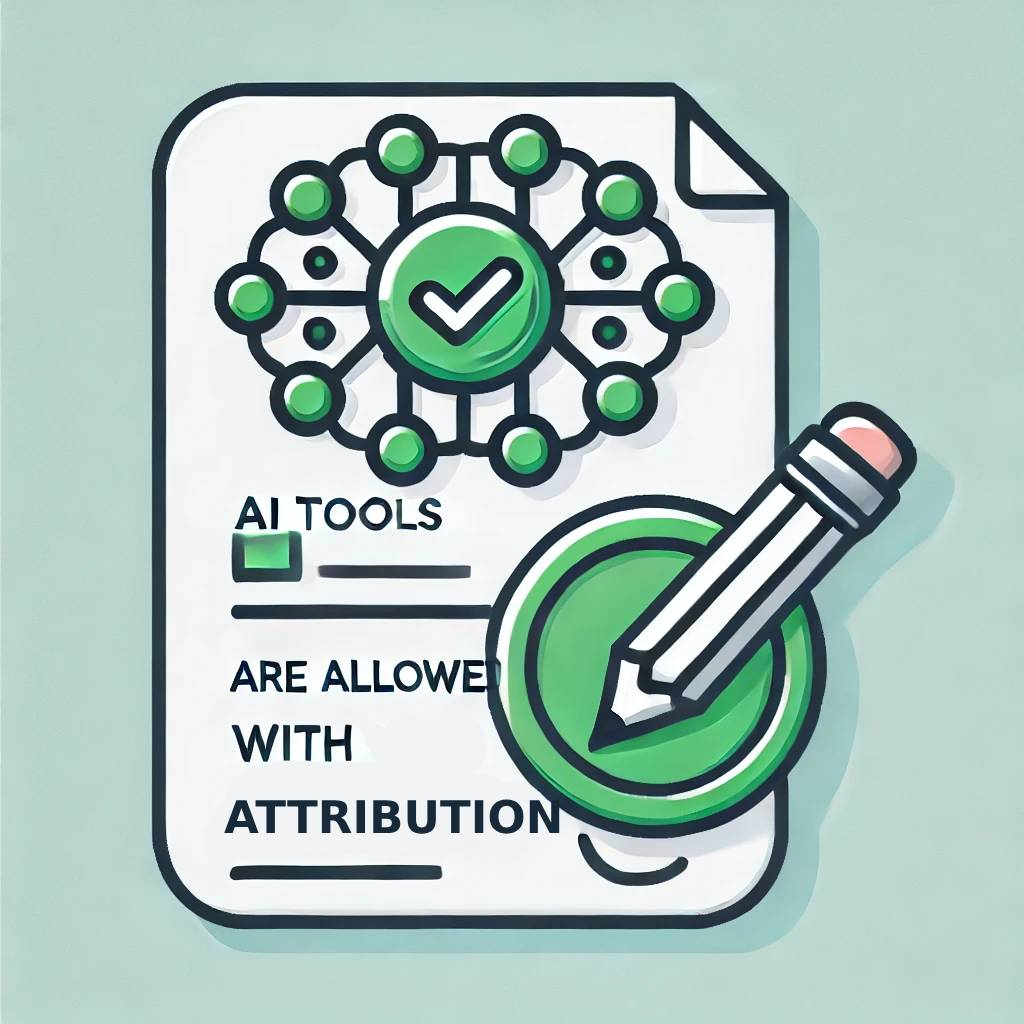
\includegraphics[width=1cm]{figs/Allowed_with_contributino.jpg}
    برای انجام این سوال به پوشه‌ی \lr{HW2\_TM} مراجعه کرده و درون فایل نوتبوک پیوست شده، سعی کنید جاهای خالی را پر کنید. برای این سوال از تصاویری که درون همان پوشه قرار داده شده‌اند استفاده کنید.\\
    در این سوال به یکی از مسائل مهم بینایی کامپیوتر به نام تطبیق کلیشه پرداخته‌ایم. در این مسئله دو نوع ورودی به نام‌های تصویر کلیشه و تصویر جست‌وجو داریم که هدف یافتن تصویر کلیشه درون تصویر جست‌وجو و برجسته‌سازی آن با رسم مستطیل به دور شی یافته شده است. یکی از ابتدائی‌ترین روش‌های انجام این مسئله این است که تصویر جست‌وجو را به نواحی‌ای تقسیم‌بندی کرده و شباهت هر یک را با تصویر کلیشه بسنجیم. اما انجام این کار دارای چالش‌های فراوانی است اعم از: کند بودن فرایند، احتمال وجود تغییرات زیاد میان کلیشه و جست‌وجو و ... . از این رو روش های مبتنی بر شبکه‌های عصبی پیچشی برای این مسئله پیشنهاد شدند که دارای دقت عملکردی بالا در مدت زمان معقولی بودند.\\
    بیشتر کد درون نوتبوک برای شما به‌صورت آماده آورده شده است. هدف از این سوال این است که آن را مطالعه کنید و درون گزارشی توضیح دهید که شبکه‌های عصبی پیچشی درون این کد چگونه به حل این مسئله کمک کرده‌اند (از آوردن جزئیاتی مانند: نحوه‌ی محاسبه‌ی \lr{confidence}، توابع کمکی، توابع رسم نتایج، \lr{NMS} و ... بپرهیزید و تنها اشاره کنید شبکه‌های عصبی پیچشی چگونه دقت و سرعت این مسئله را افزایش داده‌اند)\\
    خرجی‌های مورد انتظار درون نوتبوک فراهم شده‌اند(15 نمره).\\
    \textcolor{blue}{
    به نوتبوک \lr{Deep4032\_HW2\_TM\_Ans.ipynb} مراجعه کنید
    }

    \item 
\includegraphics[width=1cm]{figs/Forbidden_AI.jpg}
    در این سوال قرار است برای مجموعه‌ی داده‌ی زیر برای شناسایی اعداد دست‌نویس از روی تصویر ورودی، یک شبکه‌ی عصبی پیچشی با معماری دلخواه توسعه دهید. تصاویر این مجموعه‌داده، تصاویر رنگی 64 در 64 تایی از اعداد انگلیسی 1 تا 4 هستند که باید توسط شبکه‌های عصبی پیچشی آن‌ها را شناسایی کنند. این تصاویر برچسب ندارند و از روی اسم هر فایل باید ساخته شود. در شکل \ref{fig:num_pic} نمونه‌ای از این تصاویر برای شما آورده شده است(15 نمره)\\
    
    \begin{figure}[h]
        \centering
        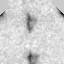
\includegraphics[width=1cm]{figs/num_pic.jpg}
        \caption{نمونه ای از تصویر عدد 4}
        \label{fig:num_pic}  
    \end{figure}

    
    می‌توانید برای این مجموعه‌داده رویه‌های مختلف داده‌افزایی را اعمال کنید.\\
    برای انجام آن به نوتبوک \lr{HW2\_CNN.ipynb} که به‌همراه سوالات پیوست گردیده است رجوع کرده و درون آن سعی کنید نواحی خالی را پر کنید.\\
    در این سوال انتظار می‌رود بتوانید مدلی را توسعه دهید که برای مجموعه‌داده‌ی آموزشی و آزمایشی (با نرخ 80 به 20 درصد از کل مجموعه‌داده با \lr{random seed = 42} برای جداسازی) به دقت بالای 90 درصد دست یابید.
    لطفا ابرپارامترهای مورد نیاز را برای احقاق نیازمندی‌های پروژه تنظیم کنید.\\
    در معماری مدل مختار هستید و می‌توانید از هر نوع مدلی استفاده کنید.\\
    پیشنهاد می‌شود از \lr{callback} هایی مانند \lr{early stopping} و \lr{learning rate scheduler} برای بهبود روند آموزش مدل استفاده کنید. (در استفاده نکردن از آن‌ها آزاد هستید.)\\
    \textbf{درون نوتبوک رویه‌ی ساخت برچسب واقعی برای هر تصویر برای شما پیاده‌سازی شده است.}\\
    \href{https://drive.google.com/drive/folders/1B66Pref_4TTUszYh5Tb08udCIIphXkl9?usp=sharing}{لینک مجموعه داده}\\
    \textcolor{blue}{
    به نوتبوک \lr{Deep4032\_HW2\_CNN\_Ans.ipynb} مراجعه کنید
    }

    \item 
\includegraphics[width=1cm]{figs/Allowed_recommended.jpg}
    مقاله \href{https://arxiv.org/pdf/1611.05431}{\lr{ResNeXt}} را مطالعه کنید و سعی کنید به دلیل موفقیت خلاقیت به کار رفته در آن خوب فکر کنید. در این سوال میخواهیم یک بلاک مشابه بلاک معرفی شده در مقاله پیاده سازی کرده و به کمک آن یک شبکه کامل بسازیم و سپس آنرا با دیتاست \lr{cifar100} آموزش دهیم.\\
    به نوتبوک \lr{Resnext.ipynb} مراجعه کنید. ابتدا یک کلاس برای بلاک \lr{resnext} طراحی کنید. سپس یک کلاس برای طراحی کامل شبکه بنویسید.در این بخش نه تنها نیازی نیست به شبکه های معرفی شده در مقاله(مانند \lr{resnext29}) وفادار باشید، بلکه توصیه میشود در طراحی خلاقیت خود را به کار بگیرید. در ساماندهی شبکه مادامی که به ایده اصلی مقاله پایبند باشید پیاده سازی شما مورد قبول است.\\
    در قسمت بعد پیش پردازش مناسب روی داده ها انجام دهید و دیتا لودرهای مورد نیاز خود را بسازید. در این قسمت تمام دانشی که در کلاس درس دراین مورد به دست آورده اید به کار بگیرید. در قسمت بعد آموزش مدل را شروع کنید. مدیریت نرخ یادگیری، نگهداری بهترین مدل و رگولاریزیشن مناسب از جمله مواردی هستند که باید به آنها توجه کافی داشته باشید. در قسمت پایانی دقت مدل را روی مجموعه دادگان تست اندازه گرفته و گزارش کنید(15 نمره).\\
    \textbf{توجه : تسلط شما به مقاله و ایده آن در زمان ارایه سنجیده خواهد شد و نیازی به گزارش نویسی برای آن نیست.}\\
    \textbf{در پاسخ این قسمت از فایل خانم میاهی‌نیا استفاده شده است}\\
    \textcolor{blue}{
    به نوتبوک \lr{Resnext.ipynb} مراجعه کنید
    }
    \item 
\includegraphics[width=1cm]{figs/Allowed_recommended.jpg}
    در این تمرین قصد داریم به مصورسازی آنچه یک شبکه پیش آموخته در مورد یک کلاس خاص فکر میکند بپردازیم. در کلاس درس یک روش برای بهینه سازی ورودی به قصد تولید تصویر بیشینه کننده احتمال تعلق به یک کلاس برای شبکه های پیش آموخته معرفی شد. در صورت نیاز به جزییات بیشتر در مورد این روش میتوانید به این \href{https://yosinski.com/deepvis}{لینک} مراجعه کنید. در این روش ابتدا یک کلاس(مثلا فلامینگو) را در نظر میگیرید و با شروع از یک تصویر تصادفی و بهینه سازی آن به تصویری میرسید که شبکه آن را متعلق به کلاس مربوطه بداند.\\
    در قسمت دوم سوال قصد داریم با استفاده از حمله \lr{fgsm} تصویری را که به نظر ما و شبکه متعلق به یک کلاس است را با کمترین تغییر به تصویری تبدیل کنیم که به نظر شبکه متعلق به کلاس مورد نظر نباشد. در صورت نیاز میتوانید این لینک را درمورد حمله \href{https://medium.com/@zachariaharungeorge/a-deep-dive-into-the-fast-gradient-sign-method-611826e34865}{\lr{fgsm}} مطالعه کنید.\\
    یک کلاس مشخص برای هر دوقسمت سوال در نظر بگیرید و تصویر به دست آمده از دو بخش را باهم مقایسه کنید(20 نمره).\\
    \textbf{در پاسخ این قسمت از فایل آقای جاوید استفاده شده است}\\
    \textcolor{blue}{
    به نوتبوک \lr{q7.ipynb} مراجعه کنید
    }

    \section*{سوال امتیازی} 
    \item 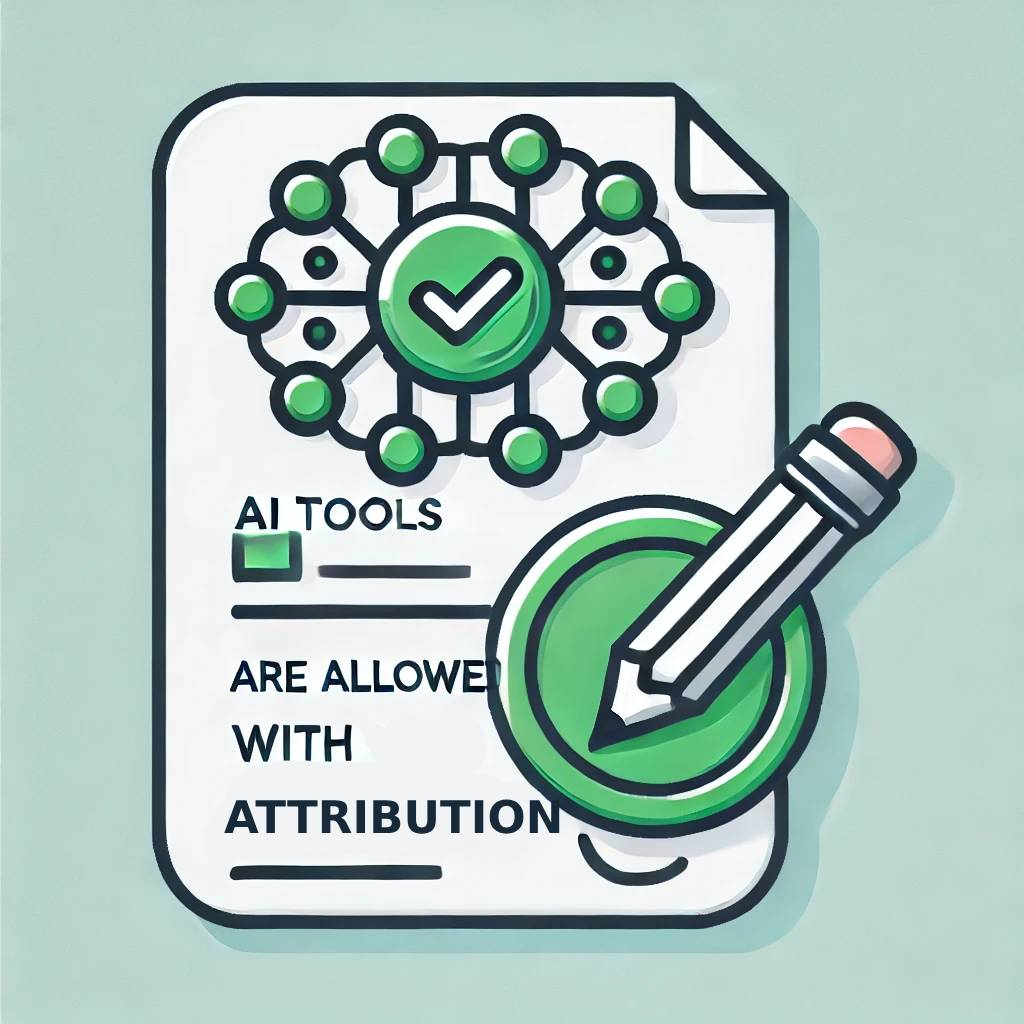
\includegraphics[width=1cm]{figs/Allowed_with_contributino.jpg}
    در این سوال قصد داریم یک مدل ناحیه‌بند معنایی  برای تصاویر \lr{X-Ray} موجود برای شناسایی نواحی پوسیدگی دندان توسعه دهیم. مسئله‌ی ناحیه‌بندی معنایی یکی از شناخته‌شده‌ترین مسائل بینایی کامپیوتر می‌باشد که در آن هدف دسته‌بندی تمامی پیکسل‌های موجود در تصویر است. شبکه‌های عصبی پیچشی با ساختاری خاص نشان‌داده‌اند که دارای قدرت مناسبی برای حل این مسئله هستند. مدل‌های \lr{SS} انواعی از شبکه‌های عصبی پیچشی هستند که ابتدا تصویر ورودی را رمزگذاری  می‌کنند تا بتوانند ویژگی‌های مناسب از تصویر ورودی را استخراج کنند. سپس در رویه‌ای به نام رمزگشایی  از روی ویژگی‌های ساخته شده، سعی می‌کنند به فضای اولیه‌ی تصویر ورودی (با همان ابعاد یکسان) بازگردند و پیکسل‌های تصویر را دسته‌بندی می‌کنند. یکی از انواع موفق شبکه‌های عصبی پیچشی در این حوزه، مدل‌های \href{https://arxiv.org/pdf/1505.04597}{\lr{Unet}} می‌باشند که ابتدا به‌صورت تدریجی تصویر را رمزگذاری کرده و سپس به‌صورت تدریجی ابعاد ویژگی‌های استخراج شده را به ابعاد تصویر اولیه بازمی‌گردانند تا عملیات دسته‌بندی را انجام دهند و در این میان تعداد مشخصی ارتباط میان رمزگذار و رمزگشا برقرار می‌کند تا بتواند از ویژگی‌های سطح پایین در این مسئله بهره ببرد. در این مسئله برچسب ورودی تصویر هم بعد تصویر ورودی با تعداد چنل 1 است که مقدار پیکسل‌های آن نشان‌دهنده‌ی کلاس آن پیکسل می‌باشد. از موارد کاربرد این مدل‌ها می‌توان به مسائل پزشکی و یافتن نواحی دارای تومور، پوسیدگی و ... از روی تصاویر پزشکی اشاره کرد.\\
    در این سوال نوع خاصی از مدل \lr{Unet} به نام \lr{ResUNet} در نظرگرفته شده است. این مدل ساختار یکسانی با مدل \lr{Unet} اصلی داراست با این تفاوت که رمزگذار آن یک مدل پیچشی \lr{Residual} است (دارای ارتباطات \lr{residual} درون رمزگذار است.). به نوتبوک \lr{HW2\_SS.ipynb} رجوع کرده و تلاش کنید با پر کردن جاهای خالی این وظیفه را به درستی پیاده‌سازی کنید.\\
    در نظر داشته باشید که از مدل فوق تنها قسمت رمزگذار آن از شما خواسته شده و باقی قسمت‌های مدل برای شما پیاده‌سازی شده‌اند.\\

    مجموعه‌داده‌ی این مسئله درون نوتبوک قرار داده شده است و با اجرای سل مربوط، مجموعه‌داده برای شما دانلود خواهد شد. اما در نظر داشته باشید که برخی از برچسب‌های این مجموعه‌داده به شدت نویزی شده‌اند که می‌تواند روند آموزش مدل شما را با مشکل روبرو کنند. برای مدیریت آن‌ها رویه‌ی متناسبی در نظر بگیرید.\\

    سعی کنید تابع هزینه (\lr{loss function}) مناسبی برای این مسئله توسعه دهید. این مسئله دسته‌بندی هر پیکسل میان دو کلاس (0 یعنی پوسیده نیست و 1 یعنی پوسیده هست) می‌باشد. یکی از توابع هزینه‌ی مناسب برای این کار \lr{BCE} می‌باشد و برای این نوع مسائل نیز استفاده می‌شود. اما استفاده از آن باید برای این مسئله بهینه شود (استفاده از تابع هزینه‌ی \lr{BCE} اولیه و بدون تغییر جواب خوبی نخواهد داد). (برای استفاده از سایر توابع هزینه‌ای که در کلاس تدریس نشده‌اند حتما منبع آن را ذکر کنید.)\\

    رسیدن به \href{https://oecd.ai/en/catalogue/metrics/dice-score#:~:text=The%20Dice%20score%20ranges%20from,of%20elements%20in%20set%20B)}{\lr{dice score}} بالای 40 درصد هم برای تصاویر آموزشی و هم آزمایشی الزامی است(20 نمره).\\
    \textcolor{blue}{
    به نوتبوک \lr{Deep4032\_HW2\_SS\_Ans.ipynb} مراجعه کنید
    }

    

\end{enumerate}



\end{document}


